\documentclass[11pt,a4paper,twoside]{article}
\usepackage[margin=1in, headheight=14pt]{geometry}
\usepackage{amsfonts,amsmath,amssymb,suetterl}
\usepackage{lmodern}
\usepackage[T1]{fontenc}
\usepackage{fancyhdr}
\usepackage{float}
\usepackage[utf8]{inputenc}
\usepackage{fontawesome}
\usepackage{enumerate}
\usepackage{xcolor}
\usepackage{hyperref}
\usepackage{tikz}
\usetikzlibrary{patterns, arrows.meta}

\DeclareUnicodeCharacter{2212}{-}

\usepackage{mathrsfs}
\usepackage[nodisplayskipstretch]{setspace}

\setstretch{1.5}
\renewcommand{\footrulewidth}{0pt}

\parindent 0ex
\setlength{\parskip}{1em}
\pagestyle{empty}

\begin{document}
    %
	\begin{singlespace}
		\begin{center}
			\Huge Queen Mary\\
			\LARGE University of London
		\end{center}
		\Large \textbf{MTH5123} \hfill \Large \textbf{Differential Equations,} \hfill \Large \textbf{Autumn 2020}\\
		\large \textbf{Coursework 3 - Week 5 - Selected Solutions} \hfill \large \textbf{W. Huang}
		\rule{\textwidth}{0.4pt}
	\end{singlespace}
	%
	\textbf{I. Practice Problems}\par
	\begin{enumerate}[\bfseries A.]
		\item Consider the initial value problem (IVP) $y^\prime = \frac{1}{2}y^{-1}\ y\in \mathbb{R},\ y(0) = 0.$
		\begin{enumerate}[\bfseries 1)]
			\item Use the Picard-Lindel\"{o}f Theorem to justify existence and uniqueness of the solution to this ODE (without exhibiting the solution)
			\item Now solve the IVP. Find and sketch all possible solutions if the solution is not unique.
			\item Change the initial condition to $y(0) = b$ where $b \neq 0$, graph the solution of this new IVP.
		\end{enumerate}
		\textbf{Solution:} (1) Since the right hand side of the ODE is $\frac{1}{2}y^{-1}$, which is not bounded in any rectangular space around an initial point at $y = 0$  (including $y(0) = 0)$, thus the first condition of Picard-Lindel\"{o}f theorem is alidated. There is no unique solution to this IVP.\par
		(2) The ODE $y^\frac{1}{2}y^{-1}$ can be solved by separation of variables, which gives two solutions $y(x) = \sqrt{x+C}$ and $y(x) = -\sqrt{x+C}$, where $x \in [c, +\infty]$.  For $y(0) = 0$, we have $C = 0$, thus the IVP has two solutions, $y_1(x) = \sqrt{x}$ and $y_2(x) = -\sqrt{x}$, where $x \in [0, +\infty]$, which can be sketched in the $xy$-plane as follow Note any IVP as $y(a) = 0$, where the
		%
		\begin{figure}[H]
			\centering
				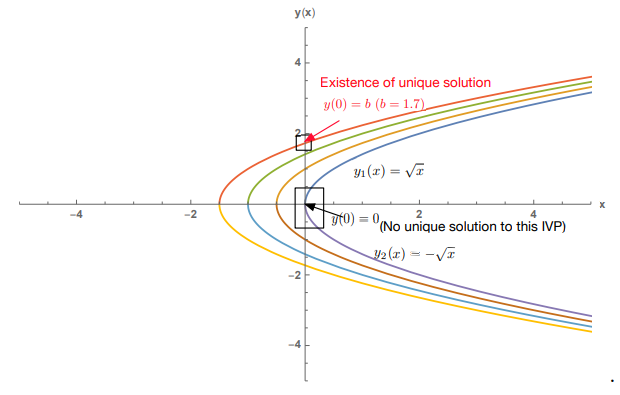
\includegraphics[width=0.75\textwidth]{figure/pdf17.PNG}
		\end{figure}
		%
		initial condition corresponds to one point in the line y = 0, will have two solutions as the case for $y(0) = 0$.\par
		(3) The initial condition $y(0) = b(b \neq 0)$, leads to $C=b^2$. And if $b>0$, the solution is $y(x) = \sqrt{x+b^2}$.  Otherwise, if $b<0,\ y(x) = -\sqrt{x+b^2}$. We can sketch the solutions as above. From the above graph, or from the Picard-Lindel\"{o}f Theorem, we can always find a rectangular space where the IVP with $y(0) = b(b \neq 0)$ has one unique solution.
		\item Assuming $x > 0$ write down the general solutions to the Euler-type equations (1)
		$$
		x^2\frac{d^y}{dx^2} - 4x\frac{dy}{dx}+6y = 0
		$$
		\textbf{Solution:} According to the general method of solving Euler-type equations we introduce the new variable $x = e^t$ and the new function $z(t)$ so that
		$$
		z(t) = y(e^t),\quad \Rightarrow \quad \frac{dz}{dt} = e^ty^\prime,\quad \frac{d^2z}{dt^2} = e^ty^\prime + e^{2t}y^{\prime\prime}
		$$
		From the above we find correspondingly that $y^\prime = e^{-t}\dot{z},\ y^{\prime\prime} e^{-2t}(\ddot{z} - \dot{z})$.  Substituting to the Euler-type equation reduces the latter to a homogeneous equation with constant coefficients.\par
		Performing the above substitutions gives in this case the equation with constant coefficients
		$$
		e^{2t}\cdot e^{-2t}\left[\frac{d^2z}{dt^2} - \frac{dz}{dt}\right]-4e^t\cdot e^{-t}\frac{dz}{dt} + 6z = 0,\quad \Rightarrow \quad \ddot{z}-5\dot{z} + 6z = 0
		$$
		The corresponding characteristic equation is $\lambda^2-5\lambda+6=0$ with the two real roots $\lambda_1 = 2$ and $\lambda_2 = 3$ so that the general solution is $z_h(t) = c_1e^{2t} + c_2e^{3t}$. The original function $y(x)$ is recovered by replacing $t = \ln x$, so that $e^{2t} = x^2,\ e^{3t} = x^3$. Finally the general solution to the original Euler equation is given by
		$$
		y_h(x) = c_1x^2 + c_2x^3.
		$$
		(2)
		$$
		x^2y^{\prime\prime} - xy^\prime - 3y = 0.
		$$
		\textbf{Solution:} Introducing the new variable by $x = e^t$ so that $y(x) \to z(t)$ and
		$$
		\frac{dy}{dx} = e^{-t}\frac{dz}{dt},\quad \frac{d^2y}{dx^2}=e^{-t}\frac{d}{dt}\left[e^{-t}\frac{dz}{dt}\right] = e^{-2t}\left[\frac{d^2z}{dt^2} - \frac{dz}{dt}\right]
		$$
		gives the equation with constant coefficients
		$$
		e^{2t}\cdot e^{-2t}\left[\frac{d^2z}{dt^2}-\frac{dz}{dt}\right] - e^t\cdot e^{-t}\frac{dz}{dt} - 3y = 0,\quad \Rightarrow \ddot{z} - 2\dot{z} - 3z = 0
		$$
		The corresponding characteristic equation is $\lambda^2 - 2\lambda - 3 = 0$ with the two real roots $\lambda_1 = −1$ and $\lambda_22 = 3$ so that the general solution is $z_h(t) = c_1e^{-t}+c_2e^{3t}$. Remembering that $t = \ln x$ so that $e^t = x$ gives $e^{-t} = 1/x,\ e^{3t} = x^3$ so that finally the general solution to the original Euler equation is given by
		$$
		y_h(x) = c_1/x + c_2x^3.
		$$
		\item Find the general solutions of the second order inhomogeneous differential equations:
		\begin{enumerate}[\bfseries 1)]
			\item $y^{\prime\prime} + 6y^\prime + 8y = -3e^{-x}$: The characteristic equation is $\lambda^2 + 6\lambda + 8 = 0$ which has two real roots: $\lambda_1 = −2$ and $\lambda_2 = −4$. The general solution to the homogeneous equation is given by $y_h(x) = c_1e^{-2x} + c_2e^{-4x}$. Since the function $e^{−x}$ is not a solution to the homogeneous equation, we may use the educated guess method and look for the particular solution of the inhomogeneous equation in the form $y_p(x) = d_0e^{-x}$. Substituting this back into the inhomogeneous equation gives on the left-hand side $e^{-x}d_0(1-6+8) = 3d_0e^{-x}$ so that to match to the right-hand side we should choose $d_0 = -1$, hence $y_p(x) = -e^{-x}$. Finally, the general solution to the inhomogeneous equation is given by
			$$
			y_p(x) = y_h(x) + y_p(x) = c_1e^{-2x} + c_2e^{-4x} - e^{-x}
			$$
			\item $y^{\prime\prime} + 7y^\prime + 6y = 10\sin 2x$: The characteristic equation is $\lambda^2 + 7\lambda + 6 = 0$ which has two real roots: $\lambda_1 = −1$ and $\lambda_2 = −6$. The general solution to the homogeneous equation is given by $y_h(x) = c_1e^{-x} + c_2e^{-6x}$. Since the function $\sin 2x$ is not a solution to the homogeneous equation, we may use the educated guess method and look for the particular solution of the inhomogeneous equation in the form $y_p(x) = A\sin 2x + B\cos 2x$, hence $y_p^\prime = = 2A \cos 2x − 2B \sin 2x$ and $y^{\prime\prime}_p = -4y_p$. Substituting this back into the inhomogeneous equation gives on the left-hand side
			\begin{gather*}
				−4(A \sin 2x + B \cos 2x) + 7 (2A \cos 2x − 2B \sin 2x) + 6(A \sin 2x + B \cos 2x)\\
				= (2A − 14B) \sin 2x + (2B + 14A) \cos 2x
			\end{gather*}
			so that to match to the right-hand side we should choose $2A − 14B = 10, 2B + 14A = 0$ so that $A = 1/10, B = −7/10$ and $y_p(x) = \frac{1}{10}(\sin 2x-7\cos 2x)$. Finally, the general solution to the inhomogeneous equation is given by the sum
			$$
			y_g(x) = c_1e^{-x} + c_2e^{-6x} + \frac{1}{10}(\sin 2x-7\cos 2x)
			$$
			\textit{Note that this differs from the two educated guess cases in the typed lecture notes. More specifically, although the roots of the characteristic equations in this example are real and the $f(x)$ has the form of sines, the educated guess still works}
		\end{enumerate}
		\item Solve the following initial value problem
		$$
		y^{\prime\prime} + 4y^\prime + 5y = 1-5x,\quad y(0) = 0,\ y^\prime(0) = -1
		$$
		\textbf{Solution:} The characteristic equation is $\lambda^2 + 4\lambda + 5 = 0$ which has two complex conjugate roots: $\lambda_1 = −2 + i$ and $\lambda_2 = −2 − i$. The general solution to the homogeneous equation is given by $y_h(x) = e^{-2x}(c_1 \cos x + c_2 \sin x)$. Since the right-hand side in the inhomogeneous equation is a polynomial, we may use the educated guess method and look for the particular solution of the inhomogeneous equation in the form $y_p(x) = d_0 + d_1x$. Substituting this back into the inhomogeneous equation gives on the left-hand side $4d_1 + 5(d_0 + d_1x) = (4d_1 + 5d_0) + 5d_1x$ so that to match to the right-hand side we should choose $4d_1 + 5d_0 = 1,\ 5d_1 = −5$, hence $y_n(x) = 1 − x$. Finally, the general solution to the inhomogeneous equation is given by $y_p(x) = e^{-2x}(c_1 \cos x + c_2 sin x) + 1 − x$ so that
		$$
		y_g^\prime(x) = e^{-2x}(-c_1 \sin x + c_2 cos x) - 2e^{-2x}(c_1\cos x + c_2\sin x) - 1
		$$
		implying
		$y(0) = c_1 + 1 = 0,\quad y^\prime (0) = c_2 - 2c_1 - 1 = −1,\quad \Rightarrow c_1 = -1,\ c_2 = -2$
		Thus, the solution to this IVP is, $y(x) = y_g(x) = e^{−2x}(- \cos x - 2 \sin x) + 1 - x$.
		\item Find the general solution of the second-order inhomogeneous differential equation
		$$
		y^{\prime\prime} + 3y^\prime + 2y = e^{-2x}\cos x.
		$$
		\textbf{Note:}
		$$
		\int e^{\alpha x}\cos \beta xdx = \frac{\beta}{\alpha^2 + \beta^2}e^{\alpha x}\left(\sin \beta x + \frac{\alpha}{\beta}\cos \beta x\right),\quad \alpha \neq \pm i\beta,
		$$
		whereas for $\alpha = \pm i\beta$ it holds
		$$
		\int e^{\pm i\beta x}\cos \beta x\, dx = \frac{x}{2}+\frac{1}{4\beta}\sin 2\beta x \mp \frac{i}{4\beta}\cos 2\beta x.
		$$
		\textbf{Solution:} The characteristic equation is $\lambda^2 + 3\lambda + 2 = 0$ with two real roots $\lambda_1 = −1,\ \lambda_2 = −2$ so the general solution of the homogeneous equation is $y_h(x) = c_1e^{-x} + c_2e^{-2x}$. As the right-hand side is not in the form allowing an educated guess we will look for a particular solution $y_p(x)$ as given by the variation of parameter method. As $\lambda_1 - \lambda_2 = 1$ we have
		$$
		y_p(x)
		= e^{-x} \int e^xe^{-2x}\cos x dx - e^{-2x} \int e^{2x}e^{-2x}\cos x dx
		= e^{-x}\int e^{-x}\cos x dx - e^{-2x} \int \cos x dx,
		$$
		where $\int \cos x dx = \sin x$ and using the formula provided
		$$
		\int e^{-x}\cos x = \frac{1}{2}e^{-x}(\sin x - \cos x)
		$$
		giving
		$$
		y_p(x) = \frac{1}{2}e^{-2x}(\sin x - \cos x) - e^{-2x}\sin x = \frac{1}{2}e^{-2x}(\sin x + \cos x).
		$$
		Finally, the general the solution of the inhomogeneous differential equation is given by
		$$
		y_g(x) = c_1e^{-x} + c_2e^{-2x}(\sin x + \cos x).
		$$
	\end{enumerate}
	%
	\textbf{II. Homework Problems}\par
	Solutions will be discussed in Week 10, session 4 (see module session schedule in Qmplus as well).\par
	%
	\textbf{III. Checking Details}\par
	We consider a problem of great importance for applications: the motion of a mass attached to an elastic string under the influence of a periodic driving force, which we have discussed in the lecture (Week 1 ) about Newton’s Second Law.\par
	%
	\textbf{Motion under periodic driving force and the resonance phenomenon}\par
	We consider differential equations for functions y(t) of an independent variable time $t \in [0,\infty)$. Let us recall that for a point mass $m$ moving along a vertical coordinate $y$ under the influence of a force $f$ Newton’s Second Law is $\text{\textbf{mass}} \times \text{\textbf{acceleration}} = \text{\textbf{force}}$. This yields a second-order differential equation
	$$
	m\ddot{y} = f(t,y),
	$$
	where we will assume for simplicity that there is no friction in the system. Thus, the force $f$ depends on time and position but not on velocity $\dot{y}$. To uniquely determine the motion of this system one has to specify initial conditions, which here are the initial value of the coordinate $y(t = 0) = y_0$ and the value of initial speed (velocity) $\dot{y}(t = 0) = v_0$. The simplest system of this type is represented by a point mass m attached to the loose end of an elastic spring of length $l$, with the other end of the spring fixed to a ceiling; see Fig. \ref{f1}. To keep our considerations as simple as possible we also neglect any additional external driving force acting on the mass. Measuring the coordinate $y$ from the ceiling downwards, the mass is then subject to a force equal to the sum of only two contributions: the position-independent \textbf{gravity force} $f_g = mg$ and the position dependent \textbf{elastic force} $f_{el} = -k(y − l)$ (Hooke’s law of elasticity).\par
	\textbf{Question:} Using the constant parameters $k,\ m,\ g,\ l$, write down the second ODE linear ODE of the position of the point mass $y$ over time $t$ for the above system. Find the
	%
	\begin{figure}[H]
		\centering
		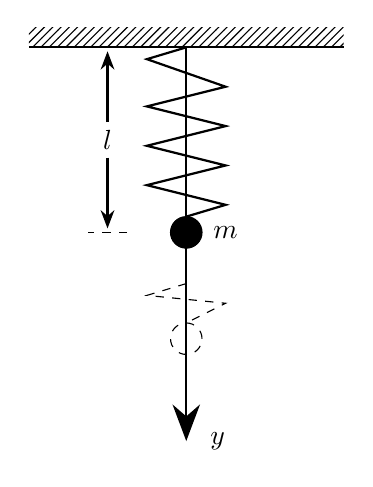
\begin{tikzpicture}
			\pattern[pattern=north east lines] (0,0) rectangle (4,.25);
			\draw[thick] (0,0) -- (4,0);
			\draw[thick,-{Stealth[scale=2]}] (2,0) -- (2,-5);
			\draw[thick] (2,0) -- (1.5,-.15) -- (2.5,-.5) -- (1.5,-.75)--(2.5,-1)--(1.5,-1.25)--(2.5, -1.5)--(1.5,-1.75)--(2.5, -2)--(2,-2.15);
			\draw[fill] (2,-2.35) circle [radius =0.2];

			\draw[dashed] (2,-3)--(1.5, -3.15)--(2.5,-3.25)--(2, -3.5);
			\draw[dashed] (2,-3.7) circle [radius =0.2];

			\draw[dashed] (1.25,-2.35) -- (0.75,-2.35);

			\node at (1,-1.175) {$l$};
			\draw[thick,-{Stealth[scale=1]}] (1,-1.4) -- (1,-2.3);
			\draw[thick,-{Stealth[scale=1]}] (1,-.95) -- (1,-.05);

			\node at (2.5,-2.35) {$m$};
			\node at (2.4,-5) {$y$};
		\end{tikzpicture}
		%
		\caption{Sketch of a spring-mass system.}\label{f1}
	\end{figure}
	%
	general solution to this ODE, and the solution to the IVP with the initial position and speed at $t = 0$ as $y(0) = y_0,\ \dot{y}(0) = 0$. Here, $y_0$ is a given constant number.\\
	(Hint: you first need to identify the focus variable, and independent variable. The ODE can be solved by second order linear ODE methods.)\par
	\textbf{Solution:} Equation
	$$
	m\ddot{y} = f(y, t),
	$$
	together with the respective initial conditions takes now the form (after division by $m$) $\ddot{y} = g - \frac{k}{m}(y-l),\ y(t = 0) = y_0,\ \dot{y}(t=0) = 0$. where $g$ is the gravitational acceleration and $k$ is the spring constant depending on the spring’s material.\\
	Note this is a inhomogenous second order linear ODE with constant coefficients, because we can reorganise our equation as $\ddot{y} + \frac{k}{m}y = g+\frac{k}{m}l$. We can directly solve this ODE by educated guess method or variation of parameter method.\\
	However, it is convenient to introduce the new coordinate $z = y−y_*$, where $y_* = l + \frac{mg}{k}$. The value $y_*$ can be found by setting $g - \frac{k}{m}(y-l) = 0$. Thus, the right-hand side of the ODE $\ddot{y} = g - \frac{k}{m}(y-l)$ vanish. This means that by choosing the initial position of the mass such that $y_0 = y_*$, if the initial speed (velocity) is zero and there is no driving force the mass will stay forever in this position.\par
	In the new coordinate $z$ reads
	$$
	\ddot{y} = \ddot{z}\quad \text{and}\quad \ddot{y} = g-\frac{k}{m}(y-l) = g-\frac{k}{m}(z+y_*-l) = -\frac{k}{m}z.
	$$
	After introducing the notation $\omega \equiv \sqrt{\frac{k}{m}}$ (known as the \textit{eigenfrequency} of the system), we can rewrite our IVP, $\ddot{y} = g-\frac{k}{m}(y-l),\ y(0) = y_0,\ \dot{y}(0) = 0$ in the form
	$$
	\ddot{z} + \omega^2z = 0,\ z(0) = z_0,\ \dot{z}(0) = 0.
	$$
	Again this is of the form of a standard homogenous second order ODE with constant coefficients. The associated characteristic equation is $\lambda^2 + \omega^2 = 0$, which has two purely imaginary complex conjugate roots, $\lambda_1 = i\omega,\ \lambda_2 = −i\omega$. We then have $z_h(t) = C_1 \cos(\omega t) + C_2 sin(\omega_t)$. According, the general solution to the original ODE is $y_h(x) = z_h(t) + y_* = C_1\cos (\omega t) + l + \frac{mg}{k}$. Using the initial conditions $z(0) = z_0,\ \dot{z}(0) = 0$, we have $C_1 = z_0$ and $C_2 = 0$, the solution to the I.V.P in the new coordinate is $z_h(t) = z_0\cos(\omega t)$.\par
	The special solution to the IVP in the original coordinate with $y(0) = y_0,\ \dot{y}(0) = 0$ is $y(x) = (y_0-l+\frac{mg}{k})\cos(\omega t)$. Recovering our previous statement, if the mass starts in the position $y_0 = l + \frac{mg}{k},\ y(x) = 0$ which means the mass will stay forever in this position.
\end{document}